\documentclass{scrartcl}
\usepackage{includes/mypack}
\usepackage{animate}
\usepackage{courier}
\usepackage{listings}
\usepackage{underscore}
\usepackage[utf8]{inputenc}
\definecolor{mygreen}{rgb}{0,0.6,0}
\definecolor{mygray}{rgb}{0.5,0.5,0.5}
\definecolor{mymauve}{rgb}{0.58,0,0.82}
\lstset{ %
  backgroundcolor=\color{white},   % choose the background color; you must add \usepackage{color} or \usepackage{xcolor}; should come as last argument
  basicstyle=\footnotesize\ttfamily,        % the size of the fonts that are used for the code
  breakatwhitespace=false,         % sets if automatic breaks should only happen at whitespace
  breaklines=true,                 % sets automatic line breaking
  captionpos=b,                    % sets the caption-position to bottom
  commentstyle=\color{mygreen},    % comment style
  %deletekeywords={...},            % if you want to delete keywords from the given language
  %escapeinside={\%*}{*)},          % if you want to add LaTeX within your code
  extendedchars=true,              % lets you use non-ASCII characters; for 8-bits encodings only, does not work with UTF-8
  %frame=single,	                   % adds a frame around the code
  keepspaces=true,                 % keeps spaces in text, useful for keeping indentation of code (possibly needs columns=flexible)
  keywordstyle=\color{blue},       % keyword style
  language=python,                 % the language of the code
  %morekeywords={*,...},            % if you want to add more keywords to the set
  numbers=left,                    % where to put the line-numbers; possible values are (none, left, right)
  numbersep=5pt,                   % how far the line-numbers are from the code
  numberstyle=\tiny\color{mygray}, % the style that is used for the line-numbers
  rulecolor=\color{black},         % if not set, the frame-color may be changed on line-breaks within not-black text (e.g. comments (green here))
  showspaces=false,                % show spaces everywhere adding particular underscores; it overrides 'showstringspaces'
  showstringspaces=false,          % underline spaces within strings only
  showtabs=false,                  % show tabs within strings adding particular underscores
  stepnumber=1,                    % the step between two line-numbers. If it's 1, each line will be numbered
  stringstyle=\color{mymauve},     % string literal style
  tabsize=4,	                   % sets default tabsize to 2 spaces
  %title=\lstname                   % show the filename of files included with \lstinputlisting; also try caption instead of title
}


\Autoren{Alice Bollenmiller, Andreas Wilhelm}
\VersuchLang{Realization of an native Android app using deep learning algorithms} %z.B. Ein Wichtiger Versuch
\VersuchKurz{Deep learning} %z.B. EWF
\Fach{Deep learning -  Dog Breed Classification} %z.B. Physik
\Studiengruppe{IG}
\Semester{WS 17/18}
\Betreuer{Lorenzo Servadei}
\selectlanguage{english}
\Datum{\today} %falls gewünscht auf Versuchsdatum ändern, z.B. 21. November 2012

\PDFStartpage{1} %Seite die im Reader beim Start geöffnet wird
\MyParLineSkip{0.5} %Höhe der Absätze die durch \mypar erzeugt werden: 0...1

\praeinit %Initialisierung der Styles Teil 1

%umschalter zwischen WORKMODE und FINALMODE
%im Workmode gibts kein titelblatt und kein inhaltsverzeichnis,
%sodass man sich auf die arbeit an sich konzentrieren kann,
%und das setzen schneller geht. 
%wichtig: immer mindestens dreimal setzen lassen,
%wenn auf final umgeschaltet wird, 
%damit Veweise und Inhaltsverzeichnis stimmen!!!!
\setboolean{finalmode}{true}

%Umschalter zwischen draft und normal mode
%bewirkt, dass falls eingeschaltet, alle grafiken durch rahmen
%der entsprechenden größe ersetzt und dargestellt werden.
%erhöht die performance beim setzen deutlich und verhindert ablenkung 
%beim arbeiten durch bilder.
\setboolean{draftgraphics}{false}

\usepackage{rotating}		%Bilder im Querformat (sidewaysfigure)

% Zitierung und Literaturverzeichnis
%-------------------------------------------------------------------
\usepackage{apacite}		% Zitierstil
\usepackage{natbib} 		% Erweiterte zitiermöglichkeiten 
\usepackage[fixlanguage]{babelbib}		% Übersetzung des Literaturverzeichnises und der Zitate
\selectbiblanguage{english}
%
%
%Abbildungen, Tabellen Ref mit Name
%
\newcommand{\mychapter}[1]{\chapter{#1} \label{chap:#1}}
\newcommand{\mysection}[1]{\section{#1} \label{sec:#1}}
\newcommand{\mysubsection}[1]{\subsection{#1} \label{subsec:#1}}
\newcommand{\mysubsubsection}[1]{\subsubsection{#1} \label{subsubsec:#1}}
%
\newcommand*{\chapref}[1]{\chaptername~\ref{chap:#1}}
\newcommand*{\secref}[1]{section~\ref{sec:#1}}
\newcommand*{\subsecref}[1]{section~\ref{subsec:#1}}
\newcommand*{\subsubsecref}[1]{section~\ref{subsubsec:#1}}
\newcommand*{\listref}[1]{listing~\ref{list:#1}}
\newcommand*{\figref}[1]{figure~\ref{fig:#1}}
\newcommand*{\tabref}[1]{table~\ref{tab:#1}}
\usepackage[format=plain,
      justification=raggedright,
      singlelinecheck=false]
     {caption}
     
% Colors
%-------------------------------------------------------------------
%usepackage[usenames]{color}
\definecolor{myMaroon}{rgb}{0.5,0.25,0}
\definecolor{gray}{gray}{0.9}
\definecolor{darkGray}{gray}{0.5}
\definecolor{lightGreen}{rgb}{0,0.2,0}
\definecolor{darkGreen}{rgb}{0,0.4,0}


% Listings Einbettung von Code (C/C++, Java, ...)
%-------------------------------------------------------------------
\usepackage{verbatim}		% Sorgt dafür, dass Text so dargestellt wird wie er eingegeben ist,
                            % es werden keine Leerzeichen oder Tabs entfernnt
\usepackage{moreverb}		% Erweiterte Möglichkeiten für verbatim                            
\usepackage{listings}		% Source-Code printer for LaTeX
\lstset{language=Python}    % Python
%\lstloadlanguages{[Visual]C++,[ISO]C++}
\lstset{numbers=left, numberstyle=\tiny, numbersep=-6pt,tabsize=3, stepnumber=1}
\lstset{framexleftmargin=-5mm, frame=single, rulesepcolor=\color{darkGray}}
\lstset{captionpos=b} 							% Beschriftung unter Listing
\lstset{backgroundcolor=\color{gray}}
\lstset{basicstyle=\scriptsize\ttfamily} 				% alle listings winzig drucken 
%\lstset{commentstyle=\color{green}} 			% Kommentare gruen drucken 
%\lstset{keywordstyle=\color{blue}\bfseries}		% Schlüsselwörter fett und blau
%\lstset{morekeywords={uint8_t, uint16_t, uint32_t, uint64_t, int8_t, int16_t, int32_t, int64_t,}}


\begin{document}
\postinit %Initialisierung der Styles Teil 2
%%AB HIER GEHT DIE ARBEIT LOS!

%\section{Introduction}
huhu

\begin{equation}
	\triangle u = f
\end{equation}

Huhu

%Example: Paper Outline
%    Introduction
%        Statement of the Problem
%        Definition of Terms
%        Theoretical Framework
%        Methodology
%            Type of Research
%            Respondents
%            Questionnaire
%        Hypothesis
%        Review of Related Literature
%        Scope and Limitations
%        Significance of the Study
%    Body
%        Background of the Study
%            Benefits of Breastfeeding
%            WHO Recommendations
%            The International Code of Marketing of Breast Milk Substitutes
%            The Baby-Friendly Hospital Initiative
%            The Innocenti Declaration on the Protection, Promotion and Support of Breastfeeding
%            National Situationer
%            The Milk Code
%            BFHI in the Philippines
%            Milk Code Violations
%            Formula Feeding
%            Factors Influencing the Decision Regarding Infant Feeding Method
%            Area Situationer
%        Presentation and Analysis of Data
%            Socio-economic Demographic Profile of Mothers
%            Information Regarding Current (Youngest) Infant
%            Current Infant Feeding Practices of Mothers
%                Exclusive Breastfeeding
%                Mixed Feeding
%                Formula Feeding
%            Previous Infant Feeding Practices
%            Maternal Knowledge
%            Correlation Tests
%    Conclusion
%        Concluding Statement
%            Analytical Summary
%            Thesis Reworded
%        Recommendations

\section{Introduction}
huhu

\begin{equation}
	\triangle u = f
\end{equation}

Huhu

\mysection{Methodological fundamentals}
This chapter describes the most frequently used frameworks in deep learning for developing applications. Furthermore, common models for deep learning are introduced. The chapter closes listing key requirements for an appropriate dataset which increases the quality of the training results.

	\mysubsection{Common Frameworks for Deep Learning Applications}
The demands on neural networks increase with the complexity of problems to solve. Concurrently, there's an expanding offer of deep learning frameworks with a varity of features and tools. The most common used ones are represented in the following section.

		\mysubsubsection{Tensorflow}
In 2015, the Google Brain Team introduced the most popular deep learning API Tensorflow which is an open-source library for numerical computation. Its current version 1.4.1 was released on December 8th, 2017 \citep{Tensorflow2017}. Tensorflow is primarily used for machine learning and deep neural network research. Based on the programming language Python, Tensorflow is capable of running on multiple CPUs and GPUs. Furthermore, C++ and R are supported by Tensorflow \citep{Varangaonkar2017}. Another feature is the possibility to generate models and export them as .pb file which holds the graph definition (GraphDef). The export is done by protocol buffers (protobuf) which includes tools for serializing and processing structured data. When loading a .pb file by protobuf, an graph object is created which holds a network of nodes. Each of these nodes represent an operation and the output is used as input for another operation. This concept enables an user to create self-built tensors \citep{TensorFlowModel2017}. To simplify the usability, Tensorflow developed a high-level wrapper of the native API which is called Tensorflow Slim \citep{TensorflowSlim}. Futhermore, in order to run Tensorflow on performance critical devices like e.g. mobile devices, two lightweight solutions of Tensorflow are available: Tensorflow Mobile and Tensorflow Lite. The latter one is an evolution of Tensorflow Mobile and still in developer mode. But both are predestinated for integration in mobile applications \citep{TensorFlowMobile}.

		\mysubsubsection{Keras}
In order to simplify the utilization of Tensorflow the Python based interface Keras can be configured to work on top of Tensorflow. It allows building neural networks in a simple way and is part of Tensorflow \citep{Varangaonkar2017}.

		\mysubsubsection{Caffe}
Another deep learning library is Caffe which was developed by Berkeley AI Research (BAIR). Based on C++ or Python, it focuses on modeling CNNs. An main advantage of Caffe is the offer of pretrained models available in the Caffe Model Zoo \citep{BAIR}. 

		\mysubsubsection{Torch and PyTorch}
Besides Tensorflow and Caffe, Torch is another common deep learning framework. It was developed by Facebook, Twitter and Google. Based on C/C++, Torch supports CUDA for GPU processing. Like above mentioned frameworks, Torch facilitates the building of neural networks. The Python based version of Torch is available through PyTorch \citep{Varangaonkar2017}.
		
	\mysubsection{Common Models in Deep Learning Applications}
State of the art models for image recognition in deep learning applications are based on the CNNs architecture. The most important ones are explained in this section. \\

The first model was LeNet-5 described in \citet{LeCun1998}. As shown in \figref{LeNet}, it contains seven layers in summary. These are two convolutional layers with a 5x5 filter each followed by a sub-sampling pooling layer. Two fully connected layers complete the architecture of the multilayer perceptron with its softmax function applied.\\
	
\begin{figure}[htbp]
\centering
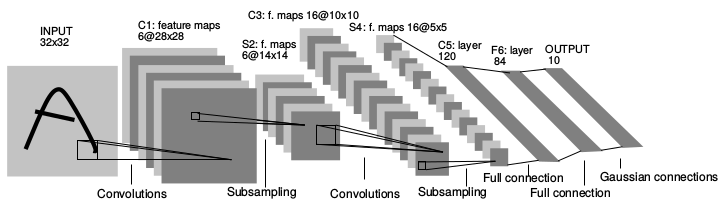
\includegraphics[width=0.8\textwidth]{includes/LeNetLecun-01a}
\caption[Model architecture of LeNet-5]{Model architecture of LeNet-5 \citep[p. 7]{LeCun1998}}
\label{fig:LeNet}
\end{figure} 

In 2012, a CNN based network called AlexNet pictured in \citet{Krizhevsky2012} wons the ImageNet Large Scale Visual Recognition Challenge (ILSVRC) for the first time (\figref{ImageNEtTop5Error}). From this time, CNN became ubiquitous.\\

\begin{figure}[htbp]
\centering
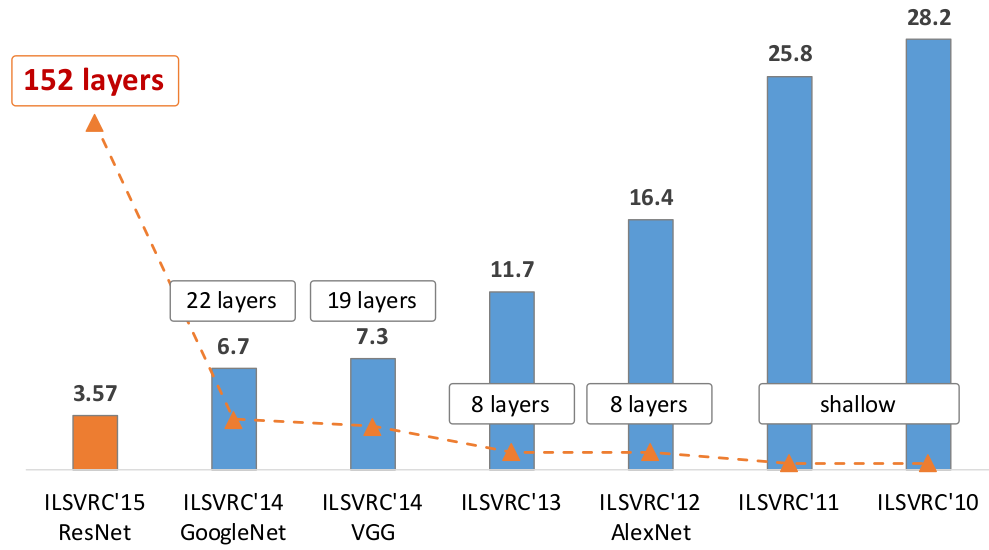
\includegraphics[width=0.8\textwidth]{includes/ImageNEtTop5Error}
\caption[ImageNet Classification top-5 error]{ImageNet Classification top-5 error (\%) \citep[p. 6]{He2016}}
\label{fig:ImageNEtTop5Error}
\end{figure}

Through its immensely improved accuracy the network created new possibilities. This CNN consists of eight layers shown in \figref{AlexNet}. The first convolutional layer has a large 11x11 filter. Furthermore, there is one layer with a 5x5 filter and another three with a 3x3 filter, so in total 5 convolutional layers. Three pooling layers and three fully connected layers complete the architecture. For the first time, a so called Rectified Linear Unit (ReLU) was used which is capable of being spread across two GPUs. \\

\begin{figure}[htbp]
\centering
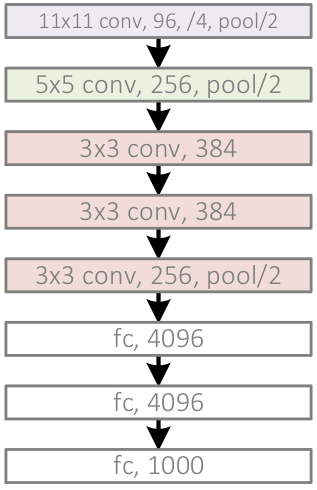
\includegraphics[width=2.5cm]{includes/AlexNet}
\caption[Model architecture of AlexNet]{Model architecture of AlexNet \citep[p. 7]{He2016}}
\label{fig:AlexNet}
\end{figure}

As shown in \figref{ImageNEtTop5Error}, the next improvements were two architectures called VGG as described in \citet{Simonyan2015} and GoogLeNet which is presented in \citet{Szegedy2014}. Introduced in 2014, they were considered as very deep neural networks. GoogLeNet is also known as \textit{InceptionV1}. \\

VGG comprises 16 or 19 layers in total (\figref{VGG19}. This network is characterized by its simplicity because it uses convolutional layers with a 3x3 filter which are stacked on top of each other. Size reduction is handled by pooling layers. At the end, there are three fully connected layers with the softmax function followed.

\begin{figure}[htbp]
\centering
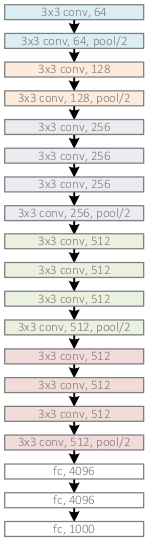
\includegraphics[width=2.5cm]{includes/VGG19}
\caption[Model architecture of VGG19]{Model architecture of VGG19 \citep[p. 8]{He2016}}
\label{fig:VGG19}
\end{figure}

Whereas, GoogLeNet has 22 layers (appendix under \subsecref{GoogLeNet - InceptionV1 architecture}) and was the final winner in 2014. At the beginning, it has two convolutional layers followed by stacked Inception modules. Such modules consists of several parallel convolutional layers with different filter size and in addition one pooling layer as shown in \figref{FH-Logo5}. On the right side of this figure a convolutional layer with a 1x1 filter is pictured which is used to reduce feature depth. At the end,the output of these modules are concatenated and taken as new input for the next layer. The network ends with one fully connected layer.\\

\begin{figure}[htbp]
\centering
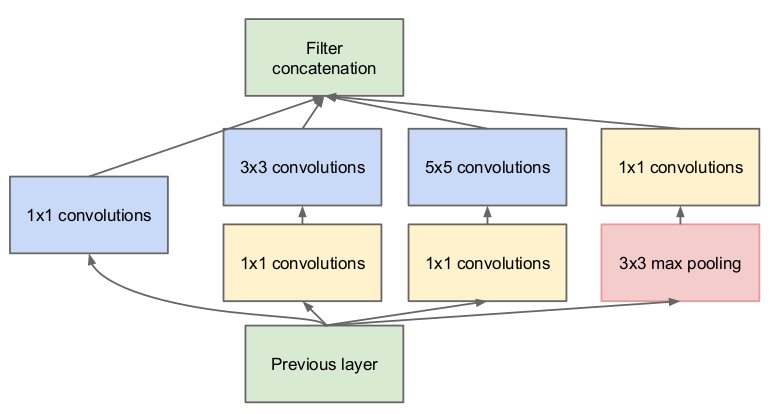
\includegraphics[width=0.7\textwidth]{includes/GoogLeNetModules}
\caption[Inception modules]{Inception modules \citep[p. 5]{Szegedy2014}}
\label{fig:FH-Logo5}
\end{figure}

Since 2015 it gets very deep with a new architecture named ResNet of \citet{HE2015}. On ILSVRC this network swept all competitiors in classification and detection. The network itself is designed as a 152 layer model. The ResNet consists of many residual network blocks (appendix under \subsecref{ResNet architecture}). Each of them has two convolutional layers with a 3x3 filter. Furthermore, there is a shortcut connection which will be used if the input and output dimension of this block are the same. \\


Especially for performance critical devices MobileNet was developed by Google as described in \citet{Howard2017}.
The network structure consists of depthwise seperable convolutional parts but also one standard convolutional layer at the beginning. The depthwise part is separated in a depthwise convolutional layer and a pointwise one which applies a 1x1 convolution. Each of this layers are followed by batchnormalisation and ReLu as shown in \figref{FH-Logo7}. In the depthwise convolutional section two convolutional layers are splitted in the one for filtering and in the one for combining. As an effect, the computation power and model size are massively reduced which results in better performance on low performance devices.

\begin{figure}[htbp]
\centering
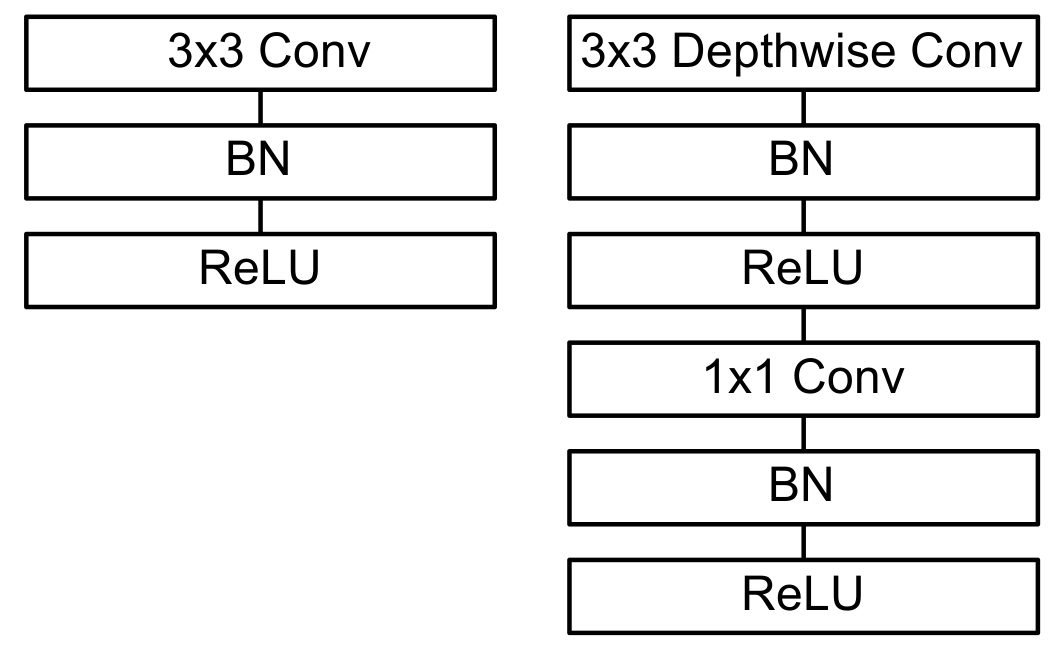
\includegraphics[width=0.4\textwidth]{includes/MobileNetArch}
\caption[Standard convolution and depthwise seperable convolution]{Standard convolution and depthwise seperable convolution \citep[p. 4]{Howard2017}}
\label{fig:FH-Logo7}
\end{figure}
 		
	\mysubsection{Key requirements for an appropriate dataset}
Supervised learning tasks such as image recognition are based on operations where an output is taken as an input for the next node. Every raw pixel input is taken to compute an intermediate representation - a vector containing all learned information about the dataset. As a consequence, the training results are only as good as the dataset itself. For better accuracy its important to train a model on a variety of images for each object which should later be classified by the model. It's recommended to take images of an object which were taken at different times, with different devices and at different places. Otherwise, the model will concentrate on other things like for example the background instead of details about the object itself. Therefore, a huge dataset is required especially for non pre-trained models. Training a model from scratch will require a huge dataset, a lot of computing power and time. Whereas pre-trained models only require a small dataset of about hundreds of images. For that reason, a pre-trained model will be used in this work \citep{TensorFlowRetrain2017}.

\mysection{Concept}
	\mysubsection{Frameworks} Alice
	- tensorflow -> why	
	\mysubsection{Model based Architectures} Andi
	 - general architectures of models -> Mobilenet, Inception
	\mysubsection{Application based Architecture} Alice


\mysection{Realization}
	\mysubsection{dataset} Andi
	\mysubsection{hardware environment} Andi
		used CPU, GPU -> NVIDIA, handys
	\mysubsection{software environment} Alice
	- Bazel, Java, Android Studio, Python, Operating System \\
 	- Android system
	\mysubsection{installation of software} Andi
 		- software environment
			\mysubsubsection{Tensorflow based on Python}
			\mysubsubsection{Tensorflow based on Bazel}
				- e.g. Workspace changes for Android SDK, msse4.2
			\mysubsubsection{Installing Android Studio and its Delevopment Kit}
				- also possible with bazel but easier Android studio (needs correct versions of sdk, ndk) \\
				- SDK, NDK \\
				- IMPORTANT: tf versions updaten (same as trained)

	\mysubsection{building the models} Alice bis Steps, Andi ab Optimierung, time GPU/CPU
	-> evtl extra subsubsection: \\
		- execution methods -> Bazel and Python (incompatible versions) \\
		- Mobilnet -> steps, optimierung \\
		- Inception -> steps, optimierung \\
		- time related differences of execution  \\
		  -> time CPUs/GPU

	\mysubsection{Output Tests and Validation} Andi
	 	- test pictures and if it works -> label image \\
	 	- validation script?! --> in Evaluierung

	\mysubsection{Implementation of an native Android App} Alice
		- list all necessary things to do (e.g. tensorflow version, Interpreter -> load Model)

	\mysubsection{Deployment and Validation} Alice



\section{Evaluation}
- prio von nierdig zu hoch \\
- regarding implementation time \\
- regarding performance \\
- regarding quality in accuracy \\
- handy perfomance? \\


\mysection{Conclusion}
At the beginning, a lot of research was done to answer the general question of 'how can a network be integrated in a mobile application and run on a performance critical device'. During the research, Tensorflow Lite was chosen as an API which enables running a network on an Android mobile phone. Because Tensorflow supports the models MobileNet and Inception specifically for mobile application usage, both were chosen. Based on this decision, both models were investigated and a comparison of both of them was incorporated into this work. After determining which framework and models are suitable for mobile applicaton support, the installation began. Because of a good documentation the installation of Tensorflow and its necessary dependencies was done quickly. Following the tutorials the models were retrained on dog images. For a first, the optimization of the models to its full degree was omitted and the focus was to include the optimized models in the mobile application for running. Therefore, Tensorflow Lite was used to convert the .pb file to a .tflite file. The conversion was conducted successfully, but the produced .tflite file caused the app to terminate. After proving the versions of all used APIs and reconverting the models several times, the app still collapsed without throwing an error. Even after optimizing, rounding, quantizing the models with different commands, the app failed to run. In addition, the tutorials and documentation are kept short on this subject. Because of this behaviour, Tensorflow Mobile was used instead of Tensorflow Lite which is still in development mode. After integration of the .pb file and its corresponding label file, the Tensorflow version had to be adapted. If adding '+' in the dependency section for Tensorflow instead of the specified version, Android Studio installs the most recent one. Futhermore, after integrating an InceptionV3 model, no results were displayed while the app was running. Therefore, the threshold was adapted to a lower value in order to display low results from the network. Next, the models were optimized to their full degree based on varying the learning rate in relation to the training steps. Afterwards, the models were comprised and loaded into the mobile application. The result are two applications, one including MobileNet and another containing InceptionV3. In the last step, the models were compared based on performance, time expenditure for producing an optimized model and quality in accuracy. Especially for the time related evaluation, marker were placed in the scripts to measure the time needed for creating the bottlenecks, training on images and evaluating an image. The expectation was that the InceptionV3 was the most accurate model, but the one with the most required performance classifying an image in the mobile application. Futhermore, the MobileNet 1.0 was expected to be the most fastest and accurate model, whereas the MobileNet 0.50 might be accurate, but slower than its successor. It turned out contrary to expectations that the MobileNet 0.50 is the most accurate one with lowest performance required (refer to \secref{Evaluation}). As a last surprise, the app was running more smoothly on the Samsung S4 device than on the newer Motorola Moto X which contains a better processor.

\mysection{Apportionment of work}
The parallel work on the entire task results in a uniform division of work. Therefore, there is no distinct apportionment of work. Here, an overview of a rough work-sharing is given by the following.

\begin{itemize}
\item Introduction (Alice)
\item Methodological fundamentals (Andreas)
\item Concept (Alice)
\item Realization (Alice and Andreas)
\item Evaluation (Andreas)
\item Conclusion (Alice and Andreas)
\end{itemize}

\clearpage
\newcounter{anhang}
\pagenumbering{Roman}
%\bibliographystyle{gerapali} % autor, jahr gerapali
\bibliographystyle{apalike} % autor, jahr
\bibliography{references}
\addcontentsline{toc}{section}{Bibliography}
\clearpage
\listoffigures
\addcontentsline{toc}{section}{List of figures}
\clearpage
\appendix
\newpage
\mysection{Appendix}

\mysubsection{Configure Bazel for Tensorflow}

\begin{lstlisting}[caption=Configure bazel for Tensorflow, label=list:configure_bazel, language=bash]
	$ cd tensorflow  # cd to the top-level directory created
	$ ./configure
	Please specify the location of python. [Default is /usr/bin/python]: /usr/bin/python3.6
	Found possible Python library paths:
	  /usr/local/lib/python3.6/dist-packages
	  /usr/lib/python3.6/dist-packages
	Please input the desired Python library path to use.  Default is [/usr/lib/python3.6/dist-packages]
	Using python library path: /usr/local/lib/python3.6/dist-packages
	Do you wish to build TensorFlow with MKL support? [y/N]
	No MKL support will be enabled for TensorFlow
	Please specify optimization flags to use during compilation when bazel option "--config=opt" is specified [Default is -march=native]:
	Do you wish to use jemalloc as the malloc implementation? [Y/n] n
	No jemalloc as malloc support will be enabled for TensorFlow.
	Do you wish to build TensorFlow with Google Cloud Platform support? [y/N] n
	No Google Cloud Platform support will be enabled for TensorFlow
	Do you wish to build TensorFlow with Hadoop File System support? [y/N] n
	No Hadoop File System support will be enabled for TensorFlow
	Do you wish to build TensorFlow with the XLA just-in-time compiler (experimental)? [y/N] n
	No XLA support will be enabled for TensorFlow
	Do you wish to build TensorFlow with Amazon S3 File System support? [Y/n]: n
	No Amazon S3 File System support will be enabled for TensorFlow.
	Do you wish to build TensorFlow with GDR support? [y/N]: n
	No GDR support will be enabled for TensorFlow.
	Do you wish to build TensorFlow with VERBS support? [y/N] n
	No VERBS support will be enabled for TensorFlow
	Do you wish to build TensorFlow with OpenCL support? [y/N] n
	No OpenCL support will be enabled for TensorFlow
	Do you wish to build TensorFlow with CUDA support? [y/N] Y
	CUDA support will be enabled for TensorFlow
	Please specify the Cuda SDK version you want to use, e.g. 7.0. [Leave empty to default to CUDA 8.0]: 8.0
	Please specify the location where CUDA 8.0 toolkit is installed. Refer to README.md for more details. [Default is /usr/local/cuda]:
	Please specify the cuDNN version you want to use. [Leave empty to default to cuDNN 6.0]: 6
	Please specify the location where cuDNN 6 library is installed. Refer to README.md for more details. [Default is /usr/local/cuda]:
	Please specify a list of comma-separated Cuda compute capabilities you want to build with.
	You can find the compute capability of your device at: https://developer.nvidia.com/cuda-gpus.
	Please note that each additional compute capability significantly increases your build time and binary size.
	[Default is: 5.2]: 5.2
	Do you want to use clang as CUDA compiler? [y/N] n
	nvcc will be used as CUDA compiler
	Please specify which gcc should be used by nvcc as the host compiler. [Default is /usr/bin/gcc]:
	Do you wish to build TensorFlow with MPI support? [y/N] n
	MPI support will not be enabled for TensorFlow
	Configuration finished
\end{lstlisting}

\begin{sidewaysfigure}
\mysubsection{Mobile Application Architecture in the form of a Class Diagram}
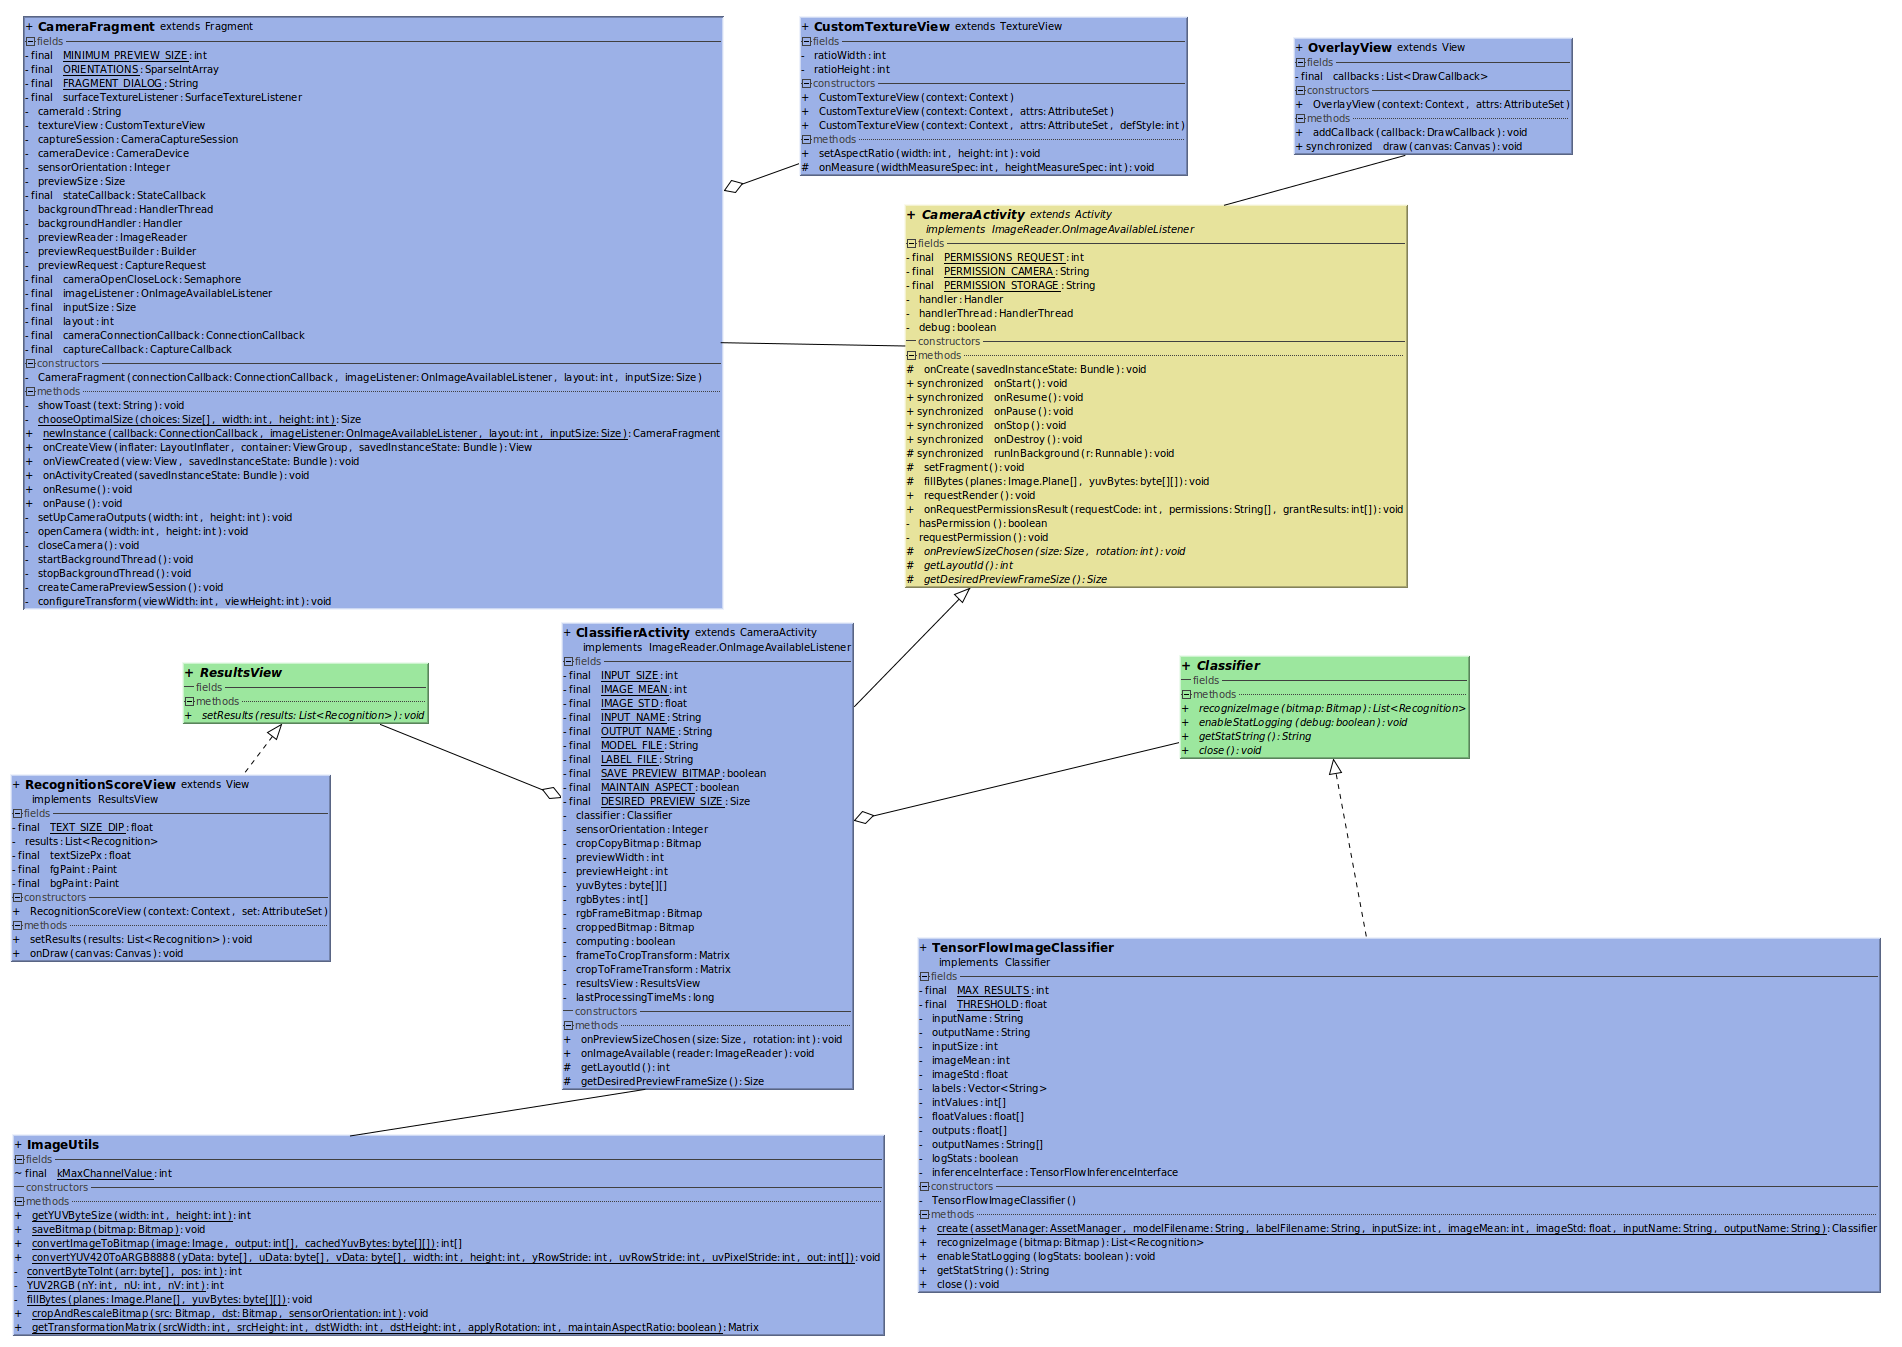
\includegraphics[width=0.95\textwidth]{includes/ClassDiagram}
\end{sidewaysfigure}
\newpage




\mysubsection{TensorBoard - optimal achieved accuracy of the different models}
\begin{figure}[htbp]
\centering
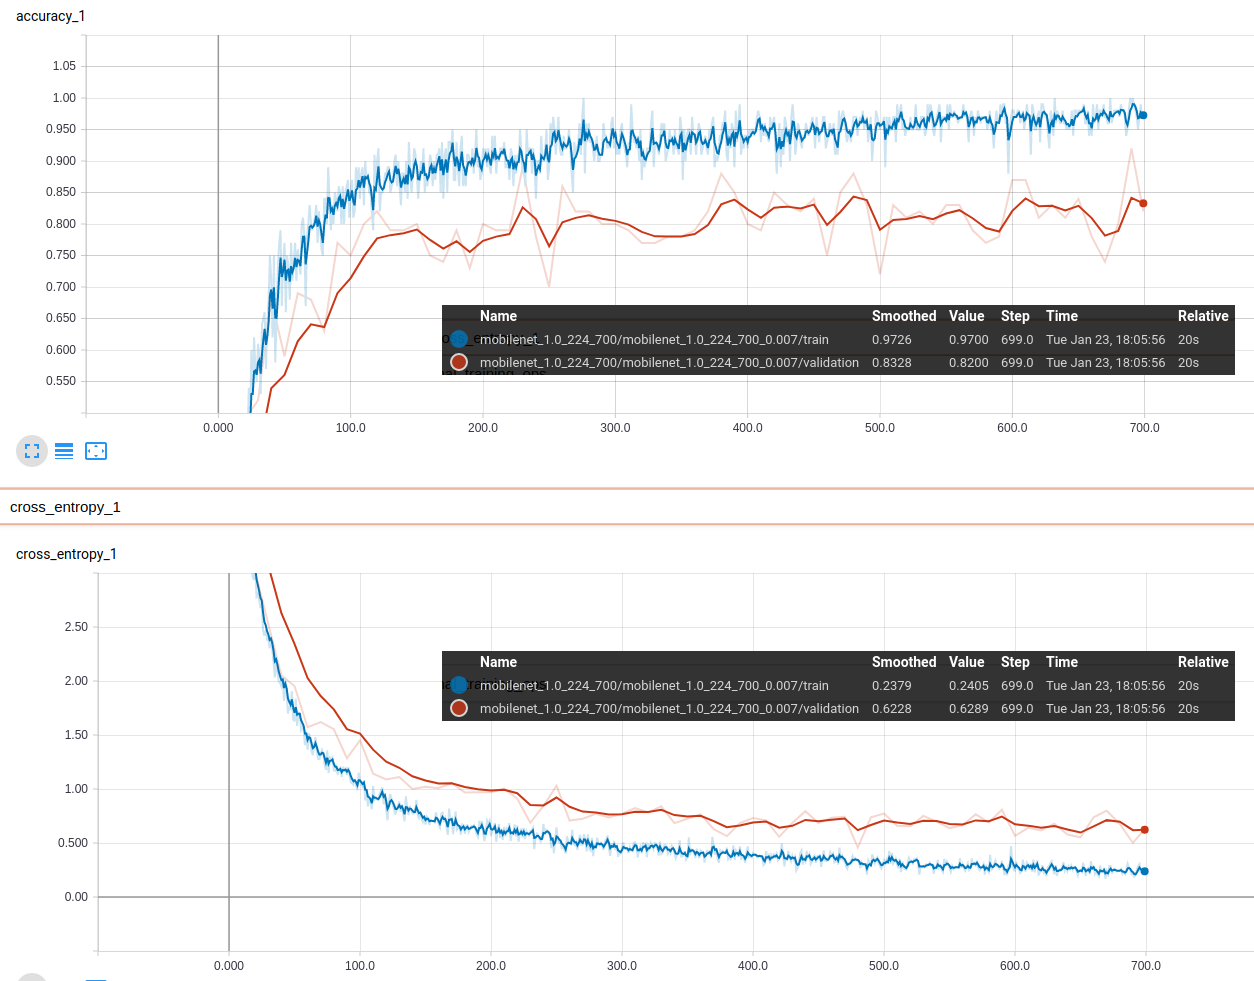
\includegraphics[width=0.95\textwidth]{includes/MobileNet05-700res}
\caption{TensorBoard - optimal achieved accuracy of MobileNet_0.5}
\label{fig:MobileNet05-700res}
\end{figure}

\begin{figure}[htbp]
\centering
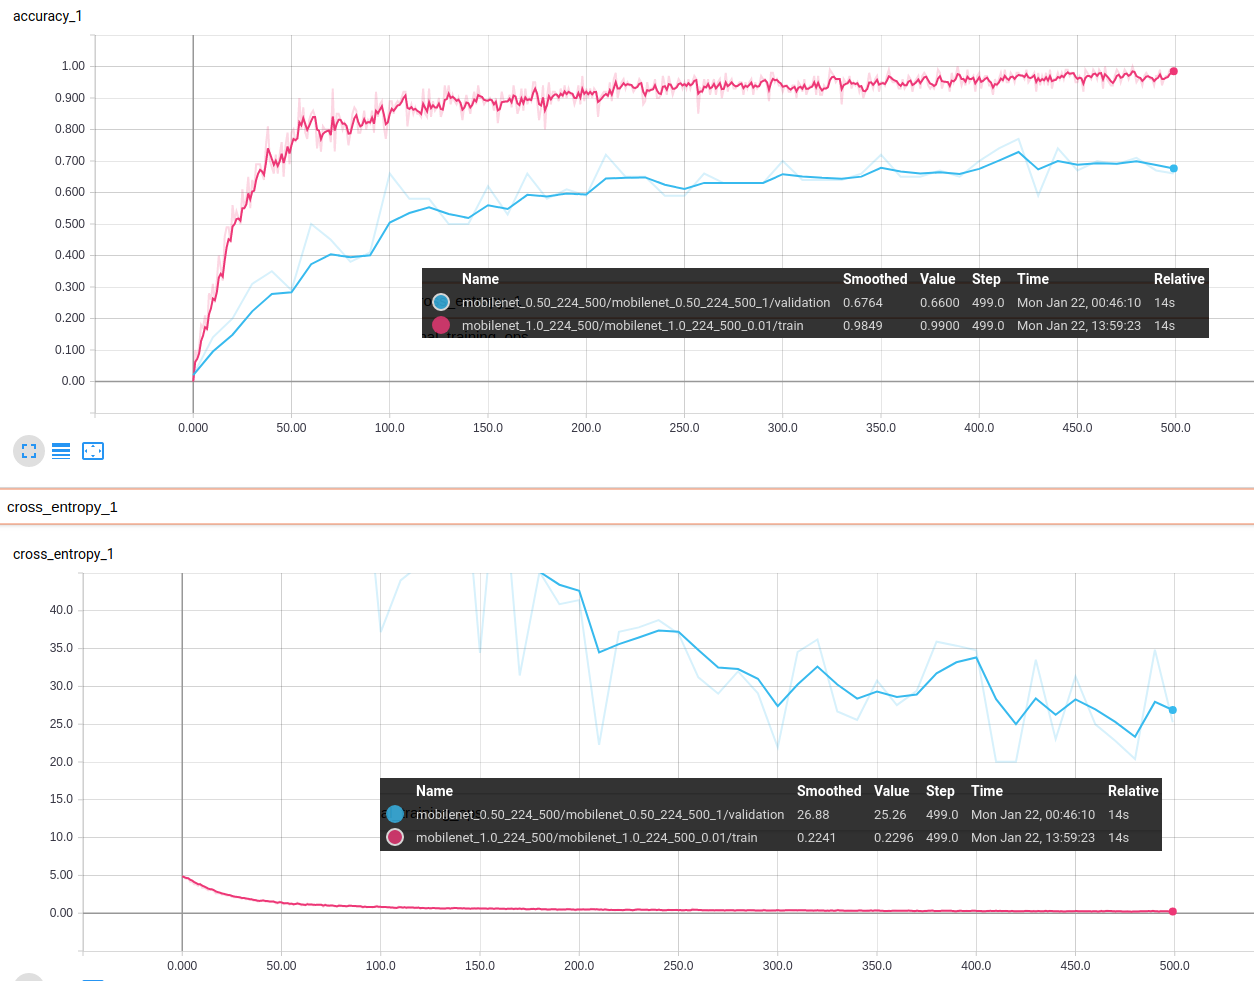
\includegraphics[width=0.95\textwidth]{includes/MobileNet10-500res}
\caption{TensorBoard - optimal achieved accuracy of MobileNet_1.0}
\label{fig:MobileNet10-500res}
\end{figure}

\begin{figure}[htbp]
\centering
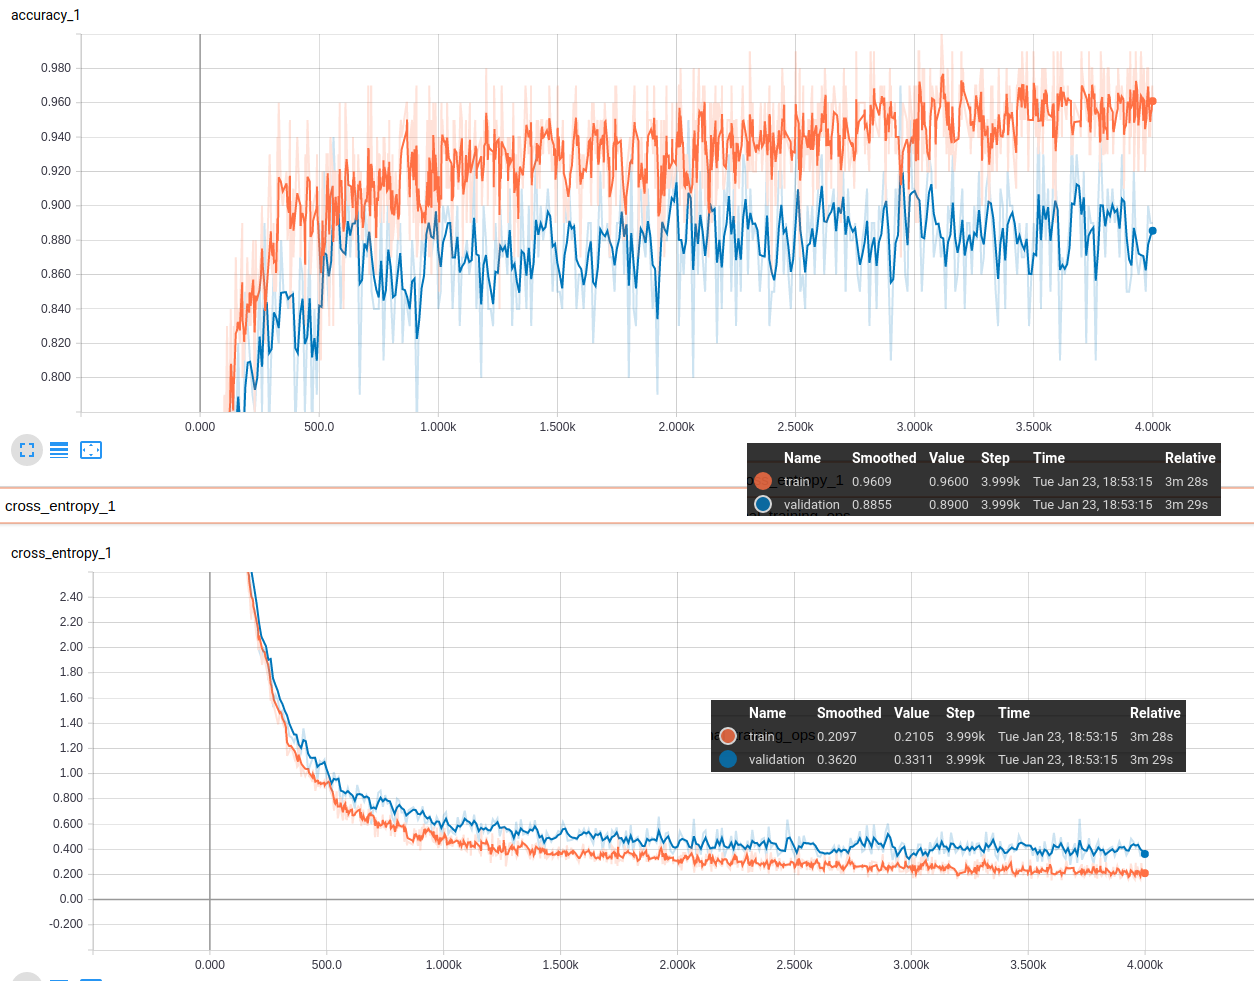
\includegraphics[width=0.95\textwidth]{includes/inception4000res}
\caption{TensorBoard - optimal achieved accuracy of InceptionV3}
\label{fig:inception4000res}
\end{figure}

\begin{figure}[htbp]
\centering
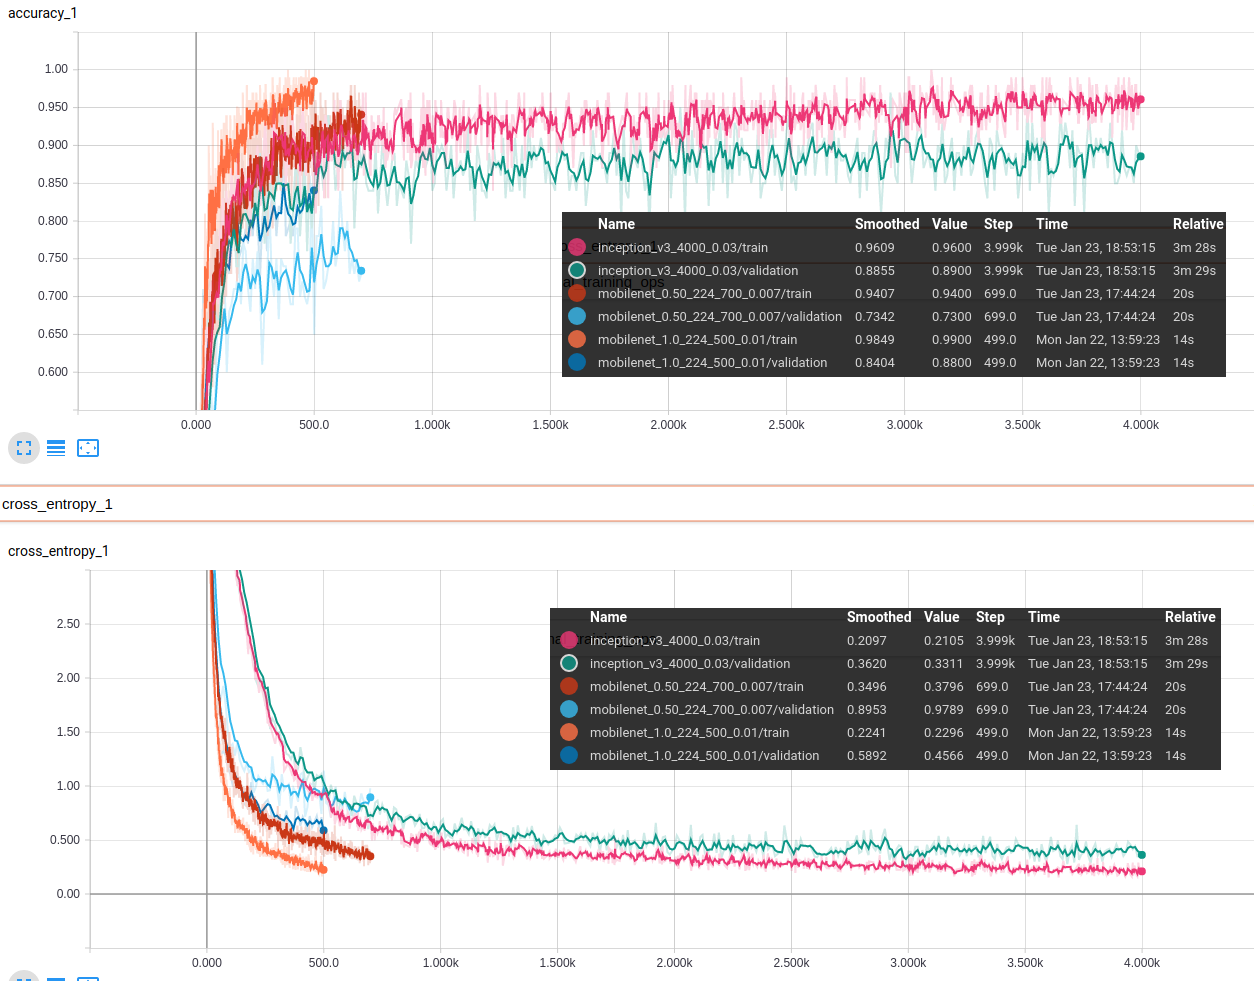
\includegraphics[width=0.95\textwidth]{includes/AllRes}
\caption{TensorBoard - optimal achieved accuracy of all models}
\label{fig:AllRes}
\end{figure}

\newpage



\mysubsection{Evaluation of optimization attempts}

\begin{table}[]
\centering
\begin{tabular}{|l|r|r|r|l}
\cline{1-4}
opt attempt & \multicolumn{1}{l|}{accuracy} & \multicolumn{1}{l|}{misclassified} & \multicolumn{1}{l|}{time to classify (App) {[}ms{]}} &  \\ \cline{1-4}
retrained & 0,566641033                   & 5                                           & 0                                &  \\ \cline{1-4}
opt1      & 0,566641033                   & 5                                           & 239,6                           &  \\ \cline{1-4}
opt2      & 0,487681977                   & 8                                           & 252,5                           &  \\ \cline{1-4}
opt3      & 0,566641033                   & 5                                           & 241,9                   &  \\ \cline{1-4}
opt4      & 0,483819713                   & 8                                           & 246,8                            &  \\ \cline{1-4}
\end{tabular}
\caption{MobileNet_0.5}
\label{tab:mobileNet05}
\end{table}

\begin{table}[]
\centering
\begin{tabular}{|l|r|r|r|l}
\cline{1-4}
opt attempt & \multicolumn{1}{l|}{accuracy} & \multicolumn{1}{l|}{misclassified} & \multicolumn{1}{l|}{time to classify (App) {[}ms{]}} &  \\ \cline{1-4}
retrained & 0,504834563                   & 7                                           & 0                                &  \\ \cline{1-4}
opt1      & 0,504834563                   & 7                                           & 316,2                            &  \\ \cline{1-4}
opt2      & 0,458024049                   & 8                                           & 310,2                           &  \\ \cline{1-4}
opt3      & 0,504834563                   & 7                                           & 323,4                            &  \\ \cline{1-4}
opt4      & 0,458474453                   & 8                                           & 320,6                           &  \\ \cline{1-4}
\end{tabular}
\caption{MobileNet_1.0}
\label{tab:mobileNet10}
\end{table}

\begin{table}[]
\centering
\begin{tabular}{|l|r|r|r|l}
\cline{1-4}
opt attempt & \multicolumn{1}{l|}{accuracy} & \multicolumn{1}{l|}{misclassified} & \multicolumn{1}{l|}{time to classify (App) {[}ms{]}} &  \\ \cline{1-4}
retrained   & 0,722748141                   & 2                                           & 0                                                    &  \\ \cline{1-4}
opt1        & 0,722748250                   & 2                                           & 1092,2                                              &  \\ \cline{1-4}
opt2        & 0,698508064                   & 3                                           & 1094,4                                               &  \\ \cline{1-4}
opt3        & 0,722748137                   & 2                                           & 1139,9                                               &  \\ \cline{1-4}
opt4        & 0,700055786                   & 3                                           & 1108,2                                               &  \\ \cline{1-4}
\end{tabular}
\caption{InceptionV3}
\label{tab:inception}
\end{table}

%%HIER ENDET DIE ARBEIT! DER REST IST KOMMENTAR MIT EIN PAAR PRAKTISCHEN FORMATIERUNGEN!!
\end{document}



%%%%%EINIGE SEHR PRAKTISCHE FORMATIERUNGSBEFEHLE UM ALLES SCHÖN UND EINHEITLICH AUSSEHEN ZU LASSEN!!%%%%%%%
%%%%%%%%%%%%%%%%%%%%%%%%%%%%%%%%%%%%%%%%%%%%%%%%%%%%%%%%%%%%%%%%%%%%%%%%%%%%%%%%%%%%%%%%%%%%%%%%%%%%%%%%%%%
%%%%%%%%%%%%%%%%%%%%%COMMENT%%%%%%%%%%%%%%%%%%%%%%COMMENT%%%%%%%%%%%%%%%%%%%%%%COMMENT%%%%%%%%%%%%%%%%%%%%%
%%%%%%%%%%%%%%%%%%%%%%%%%%%%%%%%%%%%%%%%%%%%%%%%%%%%%%%%%%%%%%%%%%%%%%%%%%%%%%%%%%%%%%%%%%%%%%%%%%%%%%%%%%%
\begin{comment}

% FORMELN UND PARAMETERBESCHREIBUNGEN
\begin{align}
\Delta \varphi = 360^\circ \cdot \frac{\Delta t}{T} = 360^\circ \cdot \Delta t \cdot f
\end{align}
wobei:
\begin{conditions} % *sternchen für zeilenübergreifende beschreibungstexte!!!
\Delta \varphi	& Phasenverschiebung \\
\Delta t		& Zeitdifferenz zwischen Eingangsspannung und gedämpfter Ausgangsspannung\\
T				& Periodendauer der Eingangsspannung \\
f				& Frequenz der Eingangsspannung
\end{conditions}

% Aufrechte griechische Buchstaben für Einheiten
\upmu
\upalpha
...etc

% BILDER EINFÜGEN
\begin{figure}[h] %t=top b=bottom h=here p =eigene page
\centering
\includegraphics[width=15cm]{media/hohlleiter}
\caption{Versuchsaufbau Hohlleiter}
\label{fig:label}
\end{figure}

% MEHRERE BILDER NEBENEINANDER
\begin{figure}[h] %t=top b=bottom h=here p =eigene page 
\flushright
\subfloat[Dispersionsrelation]{\includegraphics[width=7cm]{media/dispers}}
\subfloat[Phasen- und Gruppengeschwindigkeit]{\includegraphics[width=7cm]{media/phasgrupp}}
\end{figure}

%BILDER VOM TEXT UMFLOSSEN
\begin{wrapfigure}[10]{r}{8cm}
\centering
\includegraphics[width=7cm]{media/bragg}
\caption{\textsl{Aufbau eines Bragg-Spektrometers}}
\label{fig:bragg}
\end{wrapfigure}

%TABELLEN
\begin{table}[h]
\centering
\begin{tabular}{|c|c|}
\hline
$z$ [mm] & $\Delta z$ [mm]\\
\hline
3,3 & 0 \\
4,9 & 1,6 \\
6,5 & 1,6 \\
8,0 & 1,5 \\
\hline
\end{tabular}
\caption{Position der Minima zueinander und jeweiliger gemessener Abstand}
\label{tab:label}
\end{table}

% VERBUNDENE ZELLEN IN TABELLEN
\begin{table}[h]
\centering
\begin{tabular}{|c|c|c|c|p{1cm}p{1cm}p{1cm}p{1cm}p{1cm}p{1cm}p{1cm}|}
\hline
A & B & C & D & \multicolumn{7}{|c|}{F}  \\ \hline
\multirow{ 2}{*}{1} & 0 & 6 & 230 & 35 & 40 & 55 & 25 & 40 & 35 & \\
& 1 & 5 & 195 & 25 & 50 & 35 & 40 & 45 &  &  \\ \hline
\end{tabular}
\caption{A test caption}
\label{tab:table2}
\end{table}

% MEHRERE TABELLEN NEBENEINANDER
\begin{table}[h]
\centering

\subfloat[PVC, $d=15,0\,$mm]{
\begin{tabular}[b]{|c|c|c|}
\hline
mit Platte & ohne Platte & $\Delta s$\\
\hline
3,6 & 4,85 & 1,25\\
3,55 & 4,8 & 1,25\\
3,5 & 4,75 & 1,25\\
3,55 & 4,85 & 1,3\\
\hline
\end{tabular}
}

\subfloat[PE, $d=12,2\,$mm]{
\begin{tabular}[b]{|c|c|c|}
\hline
mit Platte & ohne Platte & $\Delta s$\\
\hline
3,5 & 4,2 & 0,7\\
3,5 & 4,25 & 0,75\\
3,5 & 4,2 & 0,7\\
\hline
\end{tabular}
}

\caption{Materialproben und zugehörige Messwerte in [cm]}
\end{table}

% FLOATS ERZWINGEN = TABELLEN UND BILDER ZWINGEND EINFÜGEN
\FloatBarrier

% ABSÄTZE MIT EINSTELLBARER UND NACHTRÄGLICH GLOBAL ÄNDERBARER DISTANZ
\mypar

% PDFs ANHÄNGEN
\includepdf[pages=-]{media/protokoll}

%BILDER UND TABELLEN REFERENZIEREN
\ref{labelname}
\pageref{labelname}

%REFERENZIERUNGSREGELN ZUR ÜBERSICHTLICHKEIT
bilder: fig:label
tabellen: tab:label
gleichungen: eq:label

\end{comment}
%%%%%%%%%%%%%%%%%%%%%%%%%%%%%%%%%%%%%%%%%%%%%%%%%%%%%%%%%%%%%%%%%%%%%%%%%%%%%%%%%%%%%%%%%%%%%%%%%%%%%%%%%%%
%%%%%%%%%%%%%%%%%%%%%COMMENT%%%%%%%%%%%%%%%%%%%%%%COMMENT%%%%%%%%%%%%%%%%%%%%%%COMMENT%%%%%%%%%%%%%%%%%%%%%
%%%%%%%%%%%%%%%%%%%%%%%%%%%%%%%%%%%%%%%%%%%%%%%%%%%%%%%%%%%%%%%%%%%%%%%%%%%%%%%%%%%%%%%%%%%%%%%%%%%%%%%%%%%
